\documentclass[11pt,a4paper]{article}
\usepackage[margin=2.2cm]{geometry}
\usepackage{amsmath,amssymb}
\usepackage{siunitx}
\usepackage{booktabs}
\usepackage{xcolor}
\usepackage{microtype}
\usepackage{enumitem}
\usepackage{tcolorbox}
\usepackage{graphicx}
\definecolor{ink}{HTML}{14231B}\definecolor{accent}{HTML}{0F3D2A}
\tcbuselibrary{skins}
\newtcolorbox{key}{colback=accent!6,colframe=accent,boxrule=0.6pt,arc=2pt,left=6pt,right=6pt,top=4pt,bottom=4pt}
\sisetup{per-mode=symbol,group-separator={\,}}
\setlength{\parindent}{0pt}\setlength{\parskip}{6pt}
\renewcommand{\arraystretch}{1.25}

\title{\textbf{Slide 7: the driver (THS4531)}\\\large Turn one wire into the two the ADC needs}
\author{ADS7057 test board v3 \quad ---\quad study notes}\date{}
\begin{document}\maketitle\vspace{-1.2em}
\section{Why two wires}
The ADS7057 measures the difference $V_\text{AINP}-V_\text{AINM}$, not a voltage to ground. Noise that reaches both inputs equally cancels. The low-pass output (LPF\_OUT) is one wire. The driver U3 makes the second wire as a mirror image of the first, around the mid-rail VOCM $=1.65$\,V.

\section{The circuit}
\begin{center}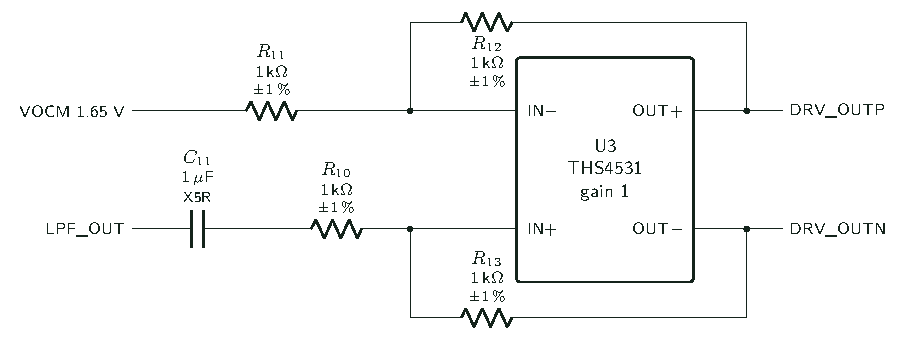
\includegraphics[width=0.98\textwidth]{s07_circuit.pdf}\end{center}
All four resistors are \SI{1}{k\ohm}. C11 blocks DC. VOCM sets the centre of the two outputs (R14, R15 divide AVDD, C13 smooths it).

\section{Derivation}
An ideal fully differential amplifier keeps its two inputs at the same voltage, $v_P=v_N=v$, and forces the average of its outputs to VOCM:
\[
\frac{v_{o+}+v_{o-}}{2}=V_\text{OCM}.
\]
Write the current balance at the two input nodes ($R=\SI{1}{k\ohm}$ for all four resistors, no current enters the amplifier):
\[
\text{node P:}\quad \frac{v_\text{in}-v}{R}+\frac{v_{o-}-v}{R}=0
\qquad
\text{node N:}\quad \frac{V_\text{OCM}-v}{R}+\frac{v_{o+}-v}{R}=0 .
\]
Subtract the second equation from the first. The $v$ terms cancel:
\[
v_\text{in}-V_\text{OCM}+v_{o-}-v_{o+}=0
\;\Rightarrow\;
\boxed{\,v_{o+}-v_{o-}=v_\text{in}-V_\text{OCM}\,}
\]
For the signal alone (deviation from DC, so $V_\text{OCM}$ does not move) the differential output equals the input: the gain is $R_{13}/R_{10}=1$. With the common-mode condition each output carries half:
\[
v_{o\pm}=V_\text{OCM}\pm\frac{v_\text{in}}{2}.
\]
\textbf{DC.} C11 is open at DC, so only R13 and R11 act. Both outputs sit at $V_\text{OCM}$ (ngspice: DRV\_OUTP and DRV\_OUTN at 1.64\,V). Nothing is amplified at DC and nothing clips.

\begin{center}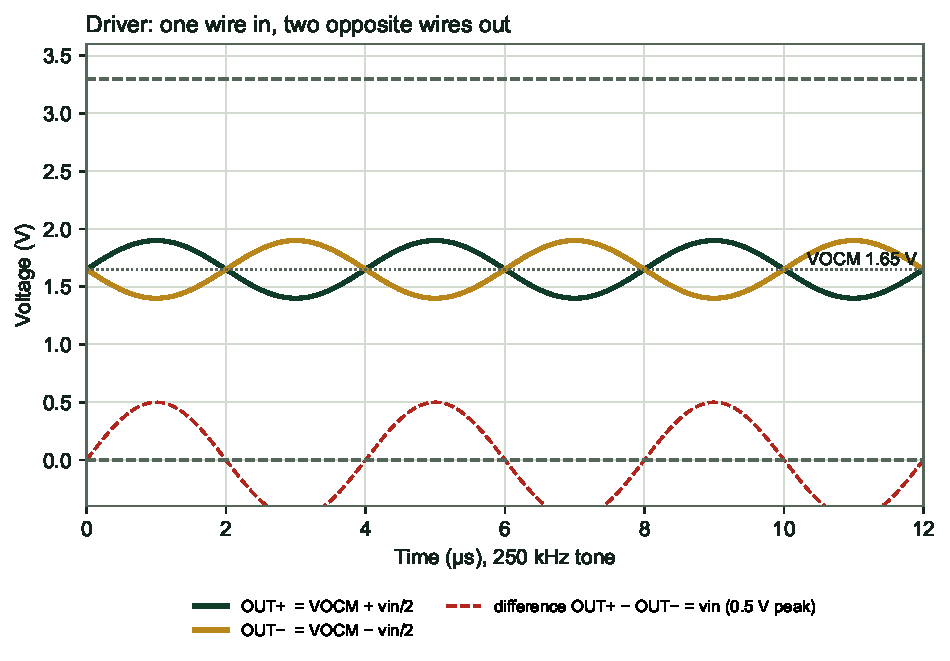
\includegraphics[width=0.8\textwidth]{s07_graph.pdf}\end{center}

\section{The input corner}
The signal source sees C11 in series with the amplifier's input resistance. The two feedback paths act on both input nodes, so the input resistance is not R10 alone. Solve node P with $v_{o+}=2v$, $v_{o-}=-2v$ (ac, outputs in opposition): $v=v_\text{in}/4$, so
\[
i_\text{in}=\frac{v_\text{in}-v}{R}=\frac{3}{4}\frac{v_\text{in}}{R}
\;\Rightarrow\;
R_\text{in}=\frac{4R}{3}=\SI{1.33}{k\ohm},\qquad
f_c=\frac{1}{2\pi R_\text{in}C_{11}}=\SI{119}{Hz}.
\]
\begin{key}
Correction to the manual (step 17): it gives \SI{159}{Hz}, which uses R10 alone. With the feedback included the corner is \SI{119}{Hz}. Both are far below the \SI{100}{kHz} band, so nothing else changes.
\end{key}

\section{Numbers to remember}
\begin{center}\begin{tabular}{lp{9cm}}
\toprule Item & Value\\\midrule
Supply and VOCM range (3.3 V) & 2.5 to 5.5 V; VOCM 0.95 to 2.3 V\\
Gain, band & differential gain 1; bandwidth far above the band\\
Event of \SI{120}{mV} at the head & about \SI{0.5}{V} between AINP and AINM\\
Load between the outputs & \SI{400}{pF} behind \SI{20}{\ohm}, the datasheet suggests about \SI{2}{pF} (open risk, slide 13)\\
\bottomrule\end{tabular}\end{center}
\end{document}
